\documentclass{ubicomp2011}
\usepackage{times}
\usepackage{url}
\usepackage{graphics}
\usepackage{color}
\usepackage[pdftex]{hyperref}
\hypersetup{%
pdftitle={Info@ITU}, pdfauthor={Egil Hansen, Jonas Rune Jensen}, pdfkeywords={ITU, BLIP, Android, Mandatory Assignment}, bookmarksnumbered, pdfstartview={FitH}, colorlinks,
citecolor=black, filecolor=black, linkcolor=black, urlcolor=black,
breaklinks=true, }
\newcommand{\comment}[1]{}
\definecolor{Orange}{rgb}{1,0.5,0}
\newcommand{\todo}[1]{\textsf{\textbf{\textcolor{Orange}{[[#1]]}}}}

%\pagenumbering{arabic}  % Arabic page numbers for submission.  Remove this line to eliminate page numbers for the camera ready copy

\begin{document}
% to make various LaTeX processors do the right thing with page size
\special{papersize=8.5in,11in}
\setlength{\paperheight}{11in}
\setlength{\paperwidth}{8.5in}
\setlength{\pdfpageheight}{\paperheight}
\setlength{\pdfpagewidth}{\paperwidth}

% use this command to override the default ACM copyright statement
% (e.g. for preprints). Remove for camera ready copy.
\toappear{}



\title{Info@ITU}
\numberofauthors{2}
\author{
  \alignauthor Egil Hansen\\
    \affaddr{IT University of Copenhagen}\\
    \email{ekri@itu.dk}
 \alignauthor Jonas Rune Jensen\\
    \affaddr{IT University of Copenhagen}\\
    \email{jrur@itu.dk}}
    
\maketitle

% \begin{abstract}
% \end{abstract}

\section{Info@ITU}
We decided to build a cloud based Info@ITU Proxy (proxy) which sits between the Info@ITU Monitor (monitor) and the phones.

\subsection{Info@ITU Proxy}
The proxy provides the following three service methods for the phones to use when interacting with the Info@ITU system:

\begin{itemize}
\item \texttt{entering?<Phones Bluetooth MAC address>}\\
This method is used by the phone to tell the system that the phone is moving into ITU and to start tracking the it.
\item \texttt{leaving?<Phones Bluetooth MAC address>}\\
This method is used by the phone to tell the system that the phone has left ITU and to stop tracking it.
\item \texttt{ping?<Phones Bluetooth MAC address>}\\
This method should be used every XX minutes, after the phone has entered into ITU, to indicate to the system that the phone is still turned on and inside ITU.
\end{itemize}

The reason why we added the \texttt{ping} method is to handle the common scenario where the phone is out of range of ITU's BLIP sensors for a longe time, i.e. when the owner is in a meeting room or lecture hall, or if the owner has turned of his phone or the phone has simply run out of power. If the proxy stops receiving pings from the phone, we assume that the phone should no longer be tracked and can save resources on the monitor.

The proxy, which is runs on Google's App Engine cloud service, also requires the user to log in with his Google ID when starting the Info@ITU App on his phone. That helps us tie a real person to a Bluetooth MAC address.

\subsubsection{Future Work}
A related feature to the \texttt{ping} method, which is not yet implemented, is a scheduled clean-up job, that searches through the list of `checked in' phones on the proxy and removes those who have not `pinged in' for XX minutes.

Push notificaitons from the proxy to the monitor would also be natural extension, since it would lower the resources required and allow the monitor to be notified almost instantly when a new phone `checks in'. In the current solution, the monitor pulls from the server every XX seconds to see if there are any new phones or phones that have left.

\subsection{Info@ITU App}

\begin{figure}[t]
\begin{center}
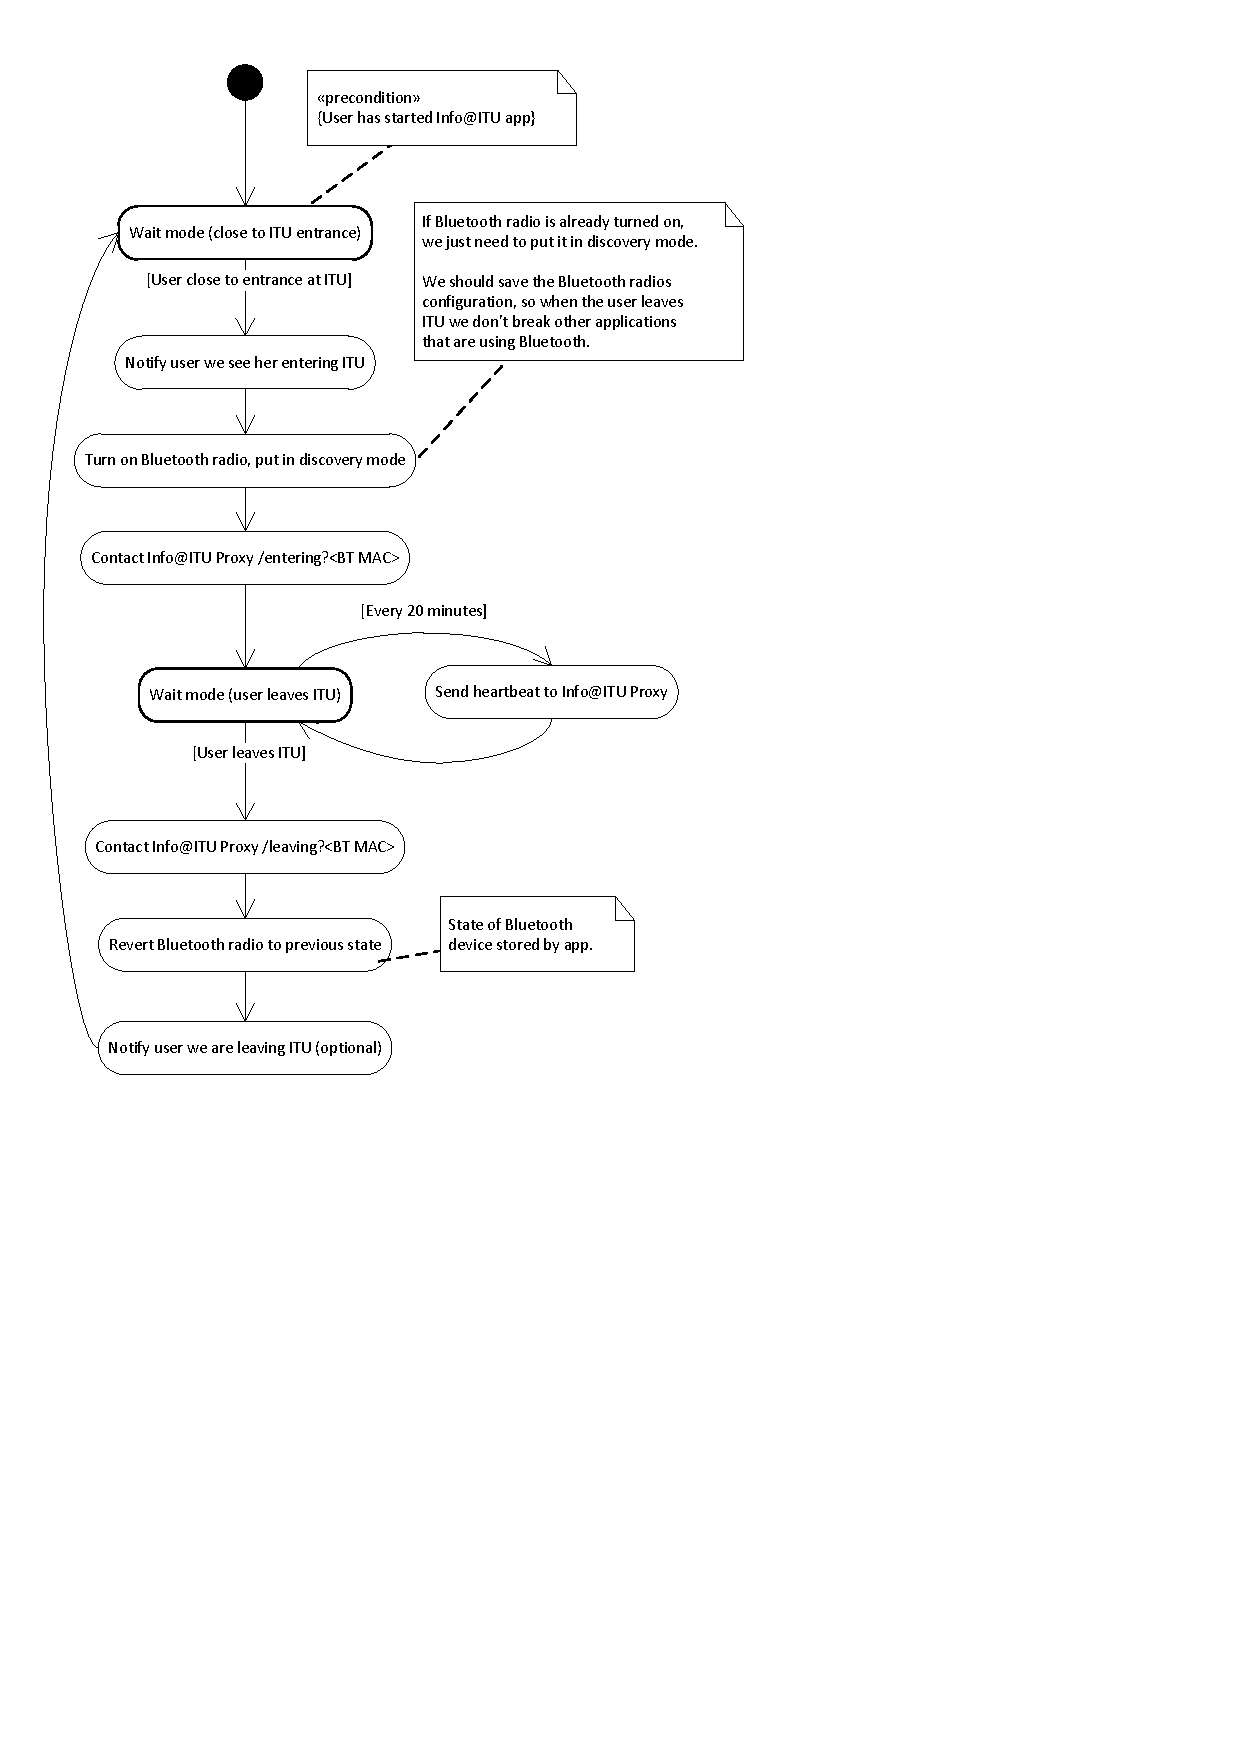
\includegraphics[width=0.95\columnwidth]{android-app-activity-diagram.pdf}
\end{center}
\caption{Activity diagram of the main service in the Info@ITU App.}
\end{figure}

%\nocite{}

\bibliographystyle{abbrv}
\bibliography{bibliography}

\end{document}